%!TEX root = ../construction.tex
% -*- root: ../construction.tex -*-

\section{Proposed System}


%%%%%%%%%%%%%%%%%%%%%%%%%%%%%%%%%%%%%%%%%%%%%%%%%%%%%%%%%%%%%%%%%%%%%%%
\subsection{System Overview}

\begin{figure}[ht!]
	\centering
    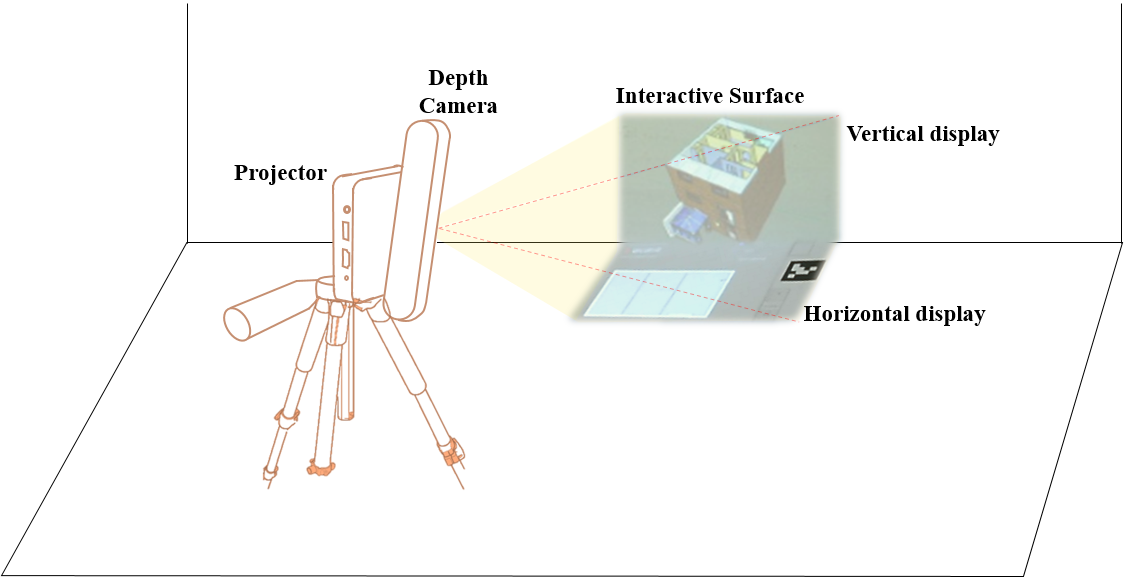
\includegraphics[width=0.8\textwidth]{3-System/overview}
	\caption{System Components}
    \label{fig:overview}
\end{figure}

제안하는 시스템은 전체적으로 그림 \ref{fig:overview}와 같이 구성된다. Interactive surface를 구성하기 위하여 한 쌍의 portable 프로젝터와 kinect 카메라 pair를 사용하였다. 이 portable 프로젝터를 통하여 현장에 필요한 정보를 제공할 수 있도록 하였다. 또한, Kinect 카메라를 이용하여 정보가 제공되는 공간을 인지함으로써 적합한 정보를 제공하거나 사용자와 상호작용할 수 있도록 하였다. 특히, 제안하는 시스템에서는 Horizontal Screen과 Vertical Screen을 구분하여 project 하도록 하였다. 이를 통하여 2차원 정보와 3차원 모델 정보를 동시에 제공함으로써 건축 현장에서 필요한 정보에 쉽게 접근하도록 하였다. Horizontal display에서는 도면위에 2D 정보를 projection 하며, Vertical display는 도면에 맞는 3D 모델을 출력한다. 두 개의 Display는 서로 동기화 되어 동작하며, 사용자는 직관적인 제스처 및 터치 상호작용을 통해 컨텐츠 제어가 가능하다.


%%%%%%%%%%%%%%%%%%%%%%%%%%%%%%%%%%%%%%%%%%%%%%%%%%%%%%%%%%%%%%%%%%%%%%%
\subsection{System Architecture}
\begin{figure}[ht!]
    \centering
    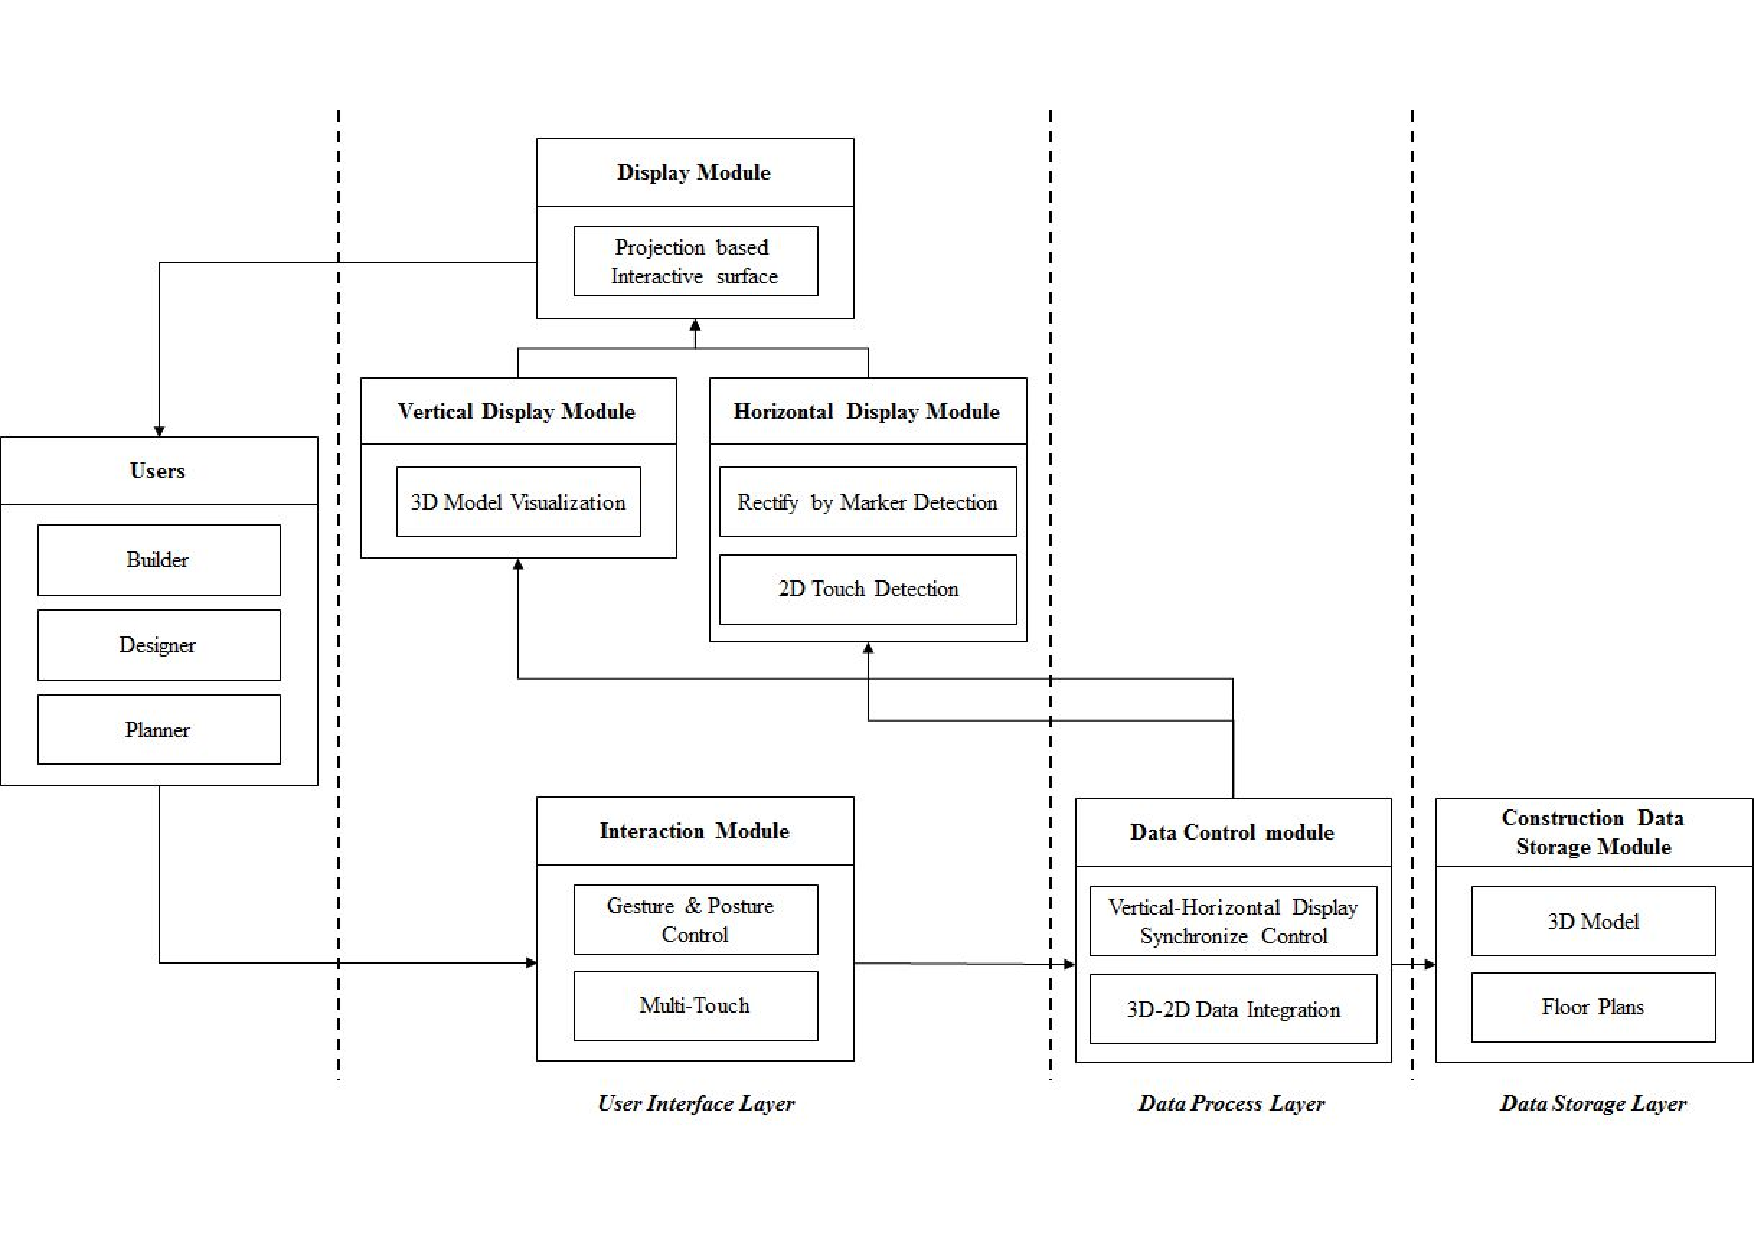
\includegraphics[width=\textwidth]{3-System/architecture_}
    \caption{The system architecture of proposed system}
    \label{fig:architecture}
\end{figure}



본 논문에서는 현장에서 필요한 정보를 이해하기 쉬운 형태로 제공하고, 현장 작업자들의 협업 지원을 위해 Projection 기반 시스템을 이용하여 시스템을 구성하였다.  Projection 기반인 Interactive Surface는 Vertical/Horizontal Display로 구성되며, 이를 이용하여 2D Floor Plan 과 3D 건축 모델의 정보를 제공한다. 또한 상호작용을 위해 제스처, 터치 기능을 지원함으로써 직관적인 제어가 가능하도록 하였다. 
그림 \ref{fig:architecture}에서 보듯이 시스템은 User Interface Layer, Data Process, Data Storage Layer 등 총 3개의 Layer로 구성되어 있다. 

\begin{itemize}
\item User Interface Layer : Vertical/Horizontal Display를 제스처, 터치 기능을 이용하여 직접적으로 제어 하며, 실시간 모델에 대한 상태 확인이 가능
\item Data Process Layer : 사용자가 입력한 건축 모델에 대한 제어를 인식하고, 결과를 Vertical/Horizontal Display에 실시간 반영하는 역할을 수행
\item Data storage Layer : 3D Model, Floor Plane와 같은 건축 정보 관리
\end{itemize}


%%%%%%%%%%%%%%%%%%%%%%%%%%%%%%%%%%%%%%%%%%%%%%%%%%%%%%%%%%%%%%%%%%%%%%%
\subsection{System Implementation}
\subsubsection{System Hardware / Hardware Implementation}
\begin{figure}[ht!]
	\centering
    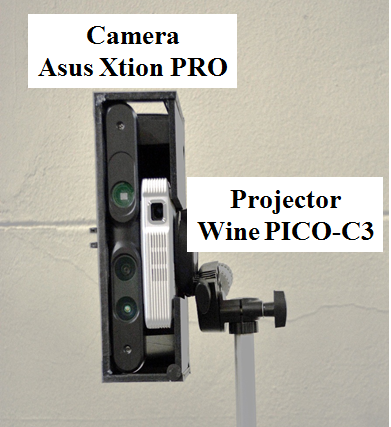
\includegraphics[width=0.4\textwidth]{3-System/hardware}
	\caption{Hardware Configuration}
    \label{fig:hardware}
\end{figure}
3D Interactive Surface의 구성을 위해 그림 \ref{fig:hardware}과 같이 Projection 기반의 하드웨어를 구성하였다. 본 연구에서 사용된 카메라는 Asus Xtion PRO, 프로젝터는 Wine PICO-C3를 사용하였으나, 다른 기종의 하드웨어를 사용하여도 무방하다. 카메라는 Horizontal Display 의 마커를 인식하고 사용자의 제스처와 터치를 인식하는데 사용되며, 프로젝터를 이용하여 영상을 출력한다. 인식하는데 카메라와 프로젝터는 캘리브레이션을 위해 서로 고정된 형태로 구성되어 있다. 이를 이용하여 마커를 인식하고, L-shape 벽면에 프로젝션 함으로써, 한 대의 프로젝터를 이용하여 Vertical/Horizontal Display 출력 및 제어가 가능하다.

%%%%%%%%%%%%%%%%
\subsubsection{Portable Multiscreen System}

제안하는 시스템은 2차원 데이터와 3차원 모델을 동시에 제공하기 위하여 Multiscreen interactive surface 기술을 이용하였다. 기존의 multiscreen interactive surface 기술은 display surface들이 고정되어 있었기 때문에 사전에 각 surface 사이의 위치 관계를 사전에 calibrate 하여 정보를 display할 수 있었다. 하지만, 제안하는 시스템은 Portable 환경을 지원하여야 하기 때문에 display surface들을 고정할 수 없고, 현장에서 즉각적으로 calibration 된 multiscreen을 제공하여야 하는 문제가 있었다. 따라서, 본 논문에서는 Image Marker 기술을 이용하여 Portable한 환경에서 실시간으로 screen을 calibrate하는 기술을 개발하였다.

\JHMEMO{calibration vs. distortion correction}

시스템의 calibration은 그림 \textcolor{red}{calibration 전/후 그림 삽입} 과 같이 Projector의 위치에 따라 찌그러져 project되는 영상을 rectify하는 기술이다. 본 논문에서는 그림 \JHMEMO{calibration 순서도 추가: 사전 calib, vertical calib, horizont calib} 와 같이 사전 Projector-Camera calibration과 Vertical Screen Calibration, Horizontal Screen Calibration 의 단계로 이루어진다. 

먼저, 사전에(offline으로) 카메라와 프로젝터 사이의 위치 관계를 보정한다. 그림 \JHMEMO{system 좌표관계 이미지}와 같이 제안하는 시스템은 IR 카메라와 RGB 카메라, 프로젝터로 구성된다. 이들은 각각 자신의 local 좌표계(coordinate system)를 가지고 있다. Offline calibration 단계에서는 이러한 센서의 intrinsic parameter와 extrinsic parameter를 계산함으로써 각 좌표계 사이에서 좌표를 변환할 수 있도록 한다. IR 카메라와 RGB 카메라 사이의 calibration은 Eq.\ref{eq:h_rgb2ir} 와 같이 checkerboard의 코너점을 각 카메라에서 인식하여 이 점의 correspondence를 계산함으로써 수행된다.
\begin{equation}
    P_{I} = H_{R \rightarrow I} P_{R}
    \label{eq:h_rgb2ir}
\end{equation}
여기에서 $P_{I}$와 $P_{R}$은 각각 IR 영상과 RGB에서의 대응된 checkerboard 코너점 집합을 의미하고, $H_{R \rightarrow I}$은 calibration결과 얻어진 RGB 영상의 좌표를 IR영상으로 변환하기 위한 행렬을 의미한다.
그리고 IR 카메라와 프로젝터 사이의 calibration은 그림 \JHMEMO{PROCAM Calibration 예제}와 같이 프로젝터로 빈 벽면에 checkboard image를 project하고 이를 RGB 좌표로 인식 한 후, 이를 IR 좌표로 변환하여 correspondence를 계산한다. 
\begin{equation}
\begin{split}
    P_{P} & = H_{R \rightarrow P} P_{R} \\
          & = H_{R \rightarrow P} H_{R \rightarrow I}^{-1} P_{I} \\
          & = H_{I \rightarrow P} P_{I}
    \label{eq:h_p2r}
\end{split}
\end{equation}
여기에서 $P_{P}$는 Projection 좌표계의 checkerboard점을 의미하고, $H_{R \rightarrow P}$와 $H_{I \rightarrow P}$는 RGB 영상과 IR 영상의 점을 Projection 이미지로 mapping 하는 변환 행렬을 의미한다. 이를 통하여 각각의 local 좌표계 좌표들은 서로 다른 좌표계로 쉽게 변환이 가능하고, 그림 \JHMEMO{calibration 결과: 손에 프로젝션 또는 checkerboard에 프로젝션}와 같이 영상을 인식하여 원하는 위치에 정보를 projection할 수 있다. 제안하는 시스템은 프로젝터와 카메라가 고정되어 있기 때문에, 이러한 프로젝터와 카메라 센서 사이의 calibration 과정은 off-line 프로세스로 단 한번만(only once) 수행된다. 

\begin{figure}[ht!]
    \centering
    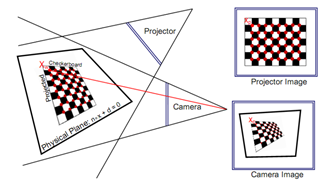
\includegraphics[width=0.4\textwidth]{3-System/calibration1}
    \caption{Projector-Camera Calibration}
    \label{fig:procam_calibration}
\end{figure}

이 후의 실시간 처리 단계에서는, projection 공간과 시스템의 위치를 분석하여 그림 \JHMEMO{rectified 결과 영상}과 같이 perspective distortion correction 을 수행한다. 이를 위하여 본 논문에서는 fiducial image marker를 이용한 distortion correction을 제안한다. fiducial image marker 는 그림 \JHMEMO{Fiducial Marker 설계}와 같이 미리 약속된 패턴의 이미지 태그이다. 미리 약속된 패턴을 인식하기 때문에, False Positive 가 낮고, ID와 pose 정보를 계산할 수 있다는 장점이 있다. 본 논문에서는 fiducial marker의 pose정보를 이용하여 distortion correction에 활용하였다. 먼저 아래와 같은 세 가지 제약사항을 가정한다.
%%% 제약사항
\begin{itemize}
    \item 프로젝션하고자 하는 평면은 평평함
    \item Fiducial marker는 직사각형
    \item Fiducial marker는 프로젝션 평면에 평행하게 위치함
\end{itemize}

가정 C3에 의하여 그림 \JHMEMO{Fiducial Marker 좌표계}에서 보는 것과 같이 Marker 좌표계는 World 좌표계와 평행하다. 
\begin{equation}
    P_M = kP_W
    \label{eq:marker2world}
\end{equation}
또한, C2에 의하여 Fiducial marker는 distortion되어 있지 않다. 따라서, Fiducial marker에 평행하게 정보를 projection하면 perspective distortion을 correct할 수 있으며, 이에 따라 marker에 평행한 Projection 좌표를 계산하는 것이 필요하다.
이는 앞의 식 \ref{eq:h_p2r} 을 이용하여 계산이 가능하다.
먼저 RGB 카메라를 이용하여 마커의 좌표를 인식한다.
\begin{equation}
    P_R' = \begin{pmatrix} 
        p_{R, 0}' \\
        p_{R, 1}' \\
        \vdots \\
        p_{R, n-1}'
    \end{pmatrix}
    \label{eq:marker2world}
\end{equation}
여기에서 







가정: 프로젝션 평면 위에 평행하게 놓임, 프로젝션 평면은 휘어있지 않고 반듯한 평면
$마커 좌표계 ~ k Projection World 좌표계$

Goal: Projection 좌표계가 나와야 함
프로세스:
  . 마커의 꼭지점 인식  
  . $마커 좌표계 - RGB 좌표계 간의 homography$
  . $마커 좌표계 ~ H R -> P  P    - projection 좌표계에 의한 마커 좌표계 계산$
  . $World 좌표계 ~ k 마커 좌표계 = H_R->P P$

\JHMEMO{predistorted 된 영상 추가}

Vertical vs. Horizontal
Vertical Screen은 고정되고, Horizontal Screen은 움직이면서 도면 제공
따라서 제안하는 시스템에서는 순서도에 따라 Vertical은 처음 1회 인식하고, Horizontal은 계속 인식함

이러한 Calibration 과정은 그림 \ref{fig:flowchart_calibration}와 같이, 사전 calibration과 realtime calibration으로 구분된다. 먼저, 사전 calibration 단계에서는, 카메라와 프로젝터 사이의 위치 관계를 보정한다. 이를 통하여 카메라를 통하여 입력되는 interactive space 에 정확하게 영상을 projection할 수 있도록 한다. 

\JHMEMO{Horizontally rotated image} 추가!

이 기술을 응용하여 MEP 정보 제공에도 사용함.
이는 벽면 등에 부착된 마커를 인식하여 Horizontal Marker 인식 모드로 진입하여 정보를 계속 제공함. (MEP 제공 영상)
























\begin{figure}[ht!]
	\centering
    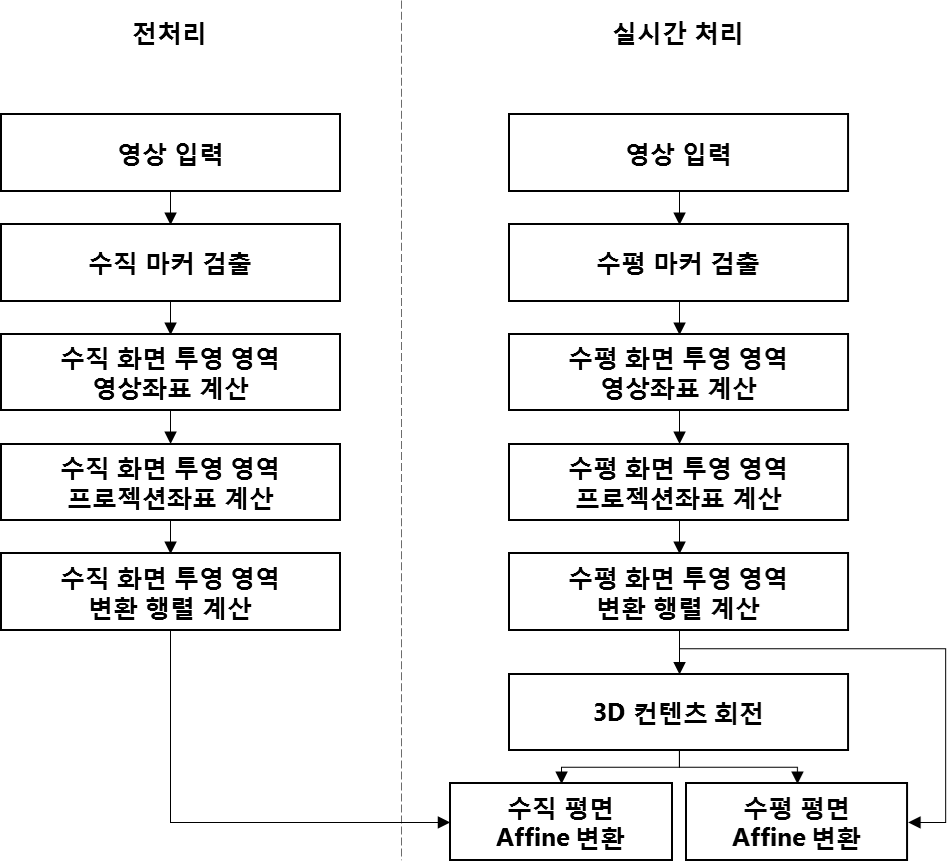
\includegraphics[width=1.0\textwidth]{3-System/flowchart_calibration}
	\caption{Calibration Flow Chart}
    \label{fig:flowchart_calibration}
\end{figure}


이 후 그림 \ref{fig:multiscreen_calibration}와 같이 Horizontal screen과 vertical screen 간의 multiscreen calibration은 마커를 이용하여 위치를 추정하였다. 
\begin{figure*}[!ht]
	\centering
        \begin{subfigure}[b]{0.8\textwidth}
            \centering
           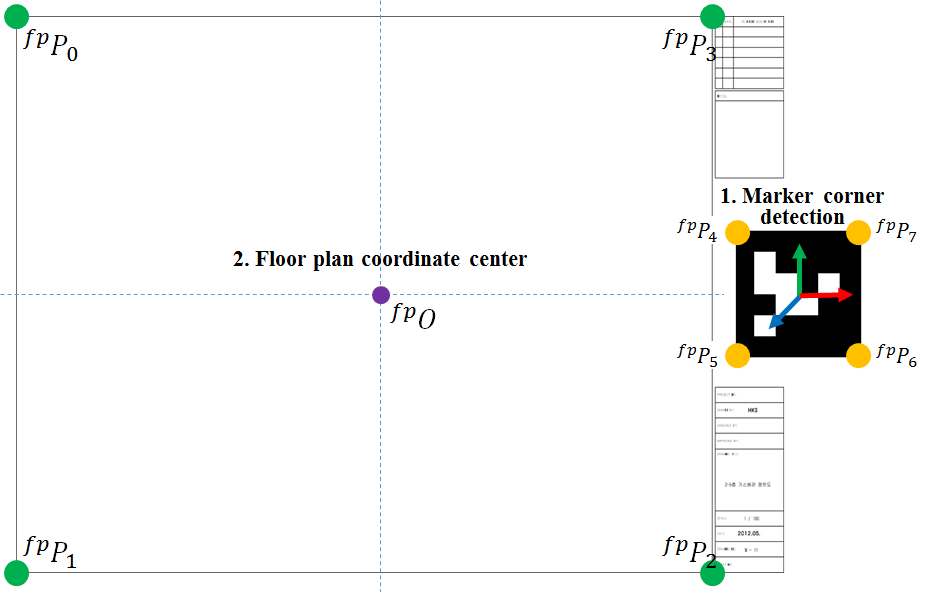
\includegraphics[width=\textwidth]{3-System/marker_calibration1}
                \caption{}
                \label{fig:marker_1}
        \end{subfigure}
        \\
        \begin{subfigure}[b]{0.8\textwidth}
	        \centering
              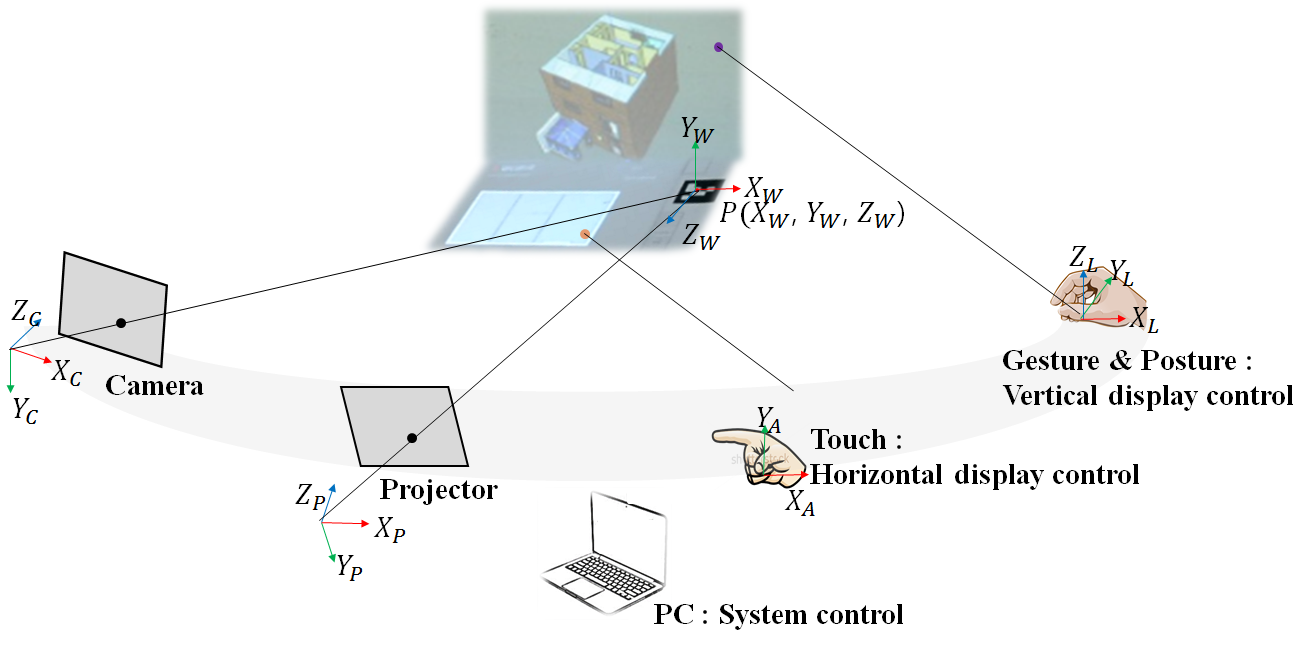
\includegraphics[width=\columnwidth]{3-System/marker_calibration2}
              \caption{}
              \label{fig:hardware}
        \end{subfigure}%
	\caption{Multiscreen Calibration}
    \label{fig:multiscreen_calibration}
\end{figure*}


위에서 설명한 캘리브레이션을 수행하게 되면 프로젝션을 위한 Vertical/Horizontal Display에 대한 위치가 결정 된다. 이러한 시스템을 이용하여 실시간 위치 추정이 가능하며, Portable 환경에서 한 대의 프로젝터를 이용하여 Multi-view를 생성하는 것을 가능하게 한다. 그림 \ref{fig:marker_calibration}은 실제 캘리브레이션을 수행하고, 마커를 이용하여 Vertical/Horizontal Display의 위치를 추정하는 단계이다. 
\begin{figure}[ht!]
	\centering
    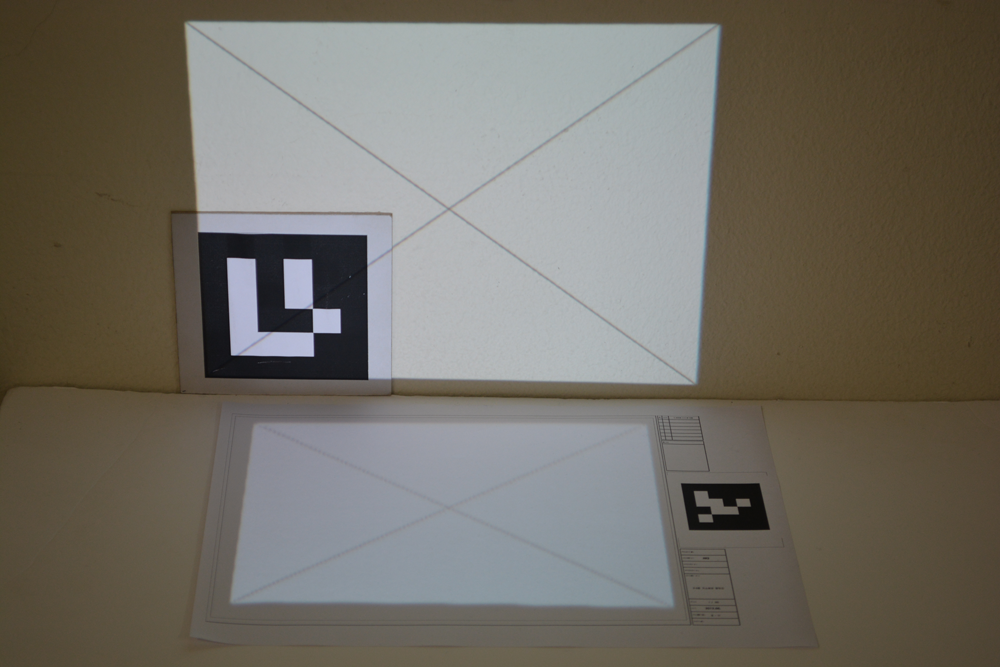
\includegraphics[width=\textwidth]{3-System/rectified}
	\caption{Marker-based Calibration}
    \label{fig:marker_calibration}
\end{figure}
입력된 영상을 기반으로 Vertical/Horizontal Display에 설정에 대한 전체적인 Flowchart는 다음과 같다. 
\textcolor{red}{Calibration Flowchart 삽입}

%%%%%%%%%%%%%%%%
\subsubsection{System Data Flow}
%%% 윤식!!! %%%


